% Auto-generated by scripts/plot_msshape.py — do not edit by hand.
% Data refreshed 2026-08-07 from local Criterion runs (Apple Silicon,
% rested machine, single-threaded: RAYON_NUM_THREADS=1,
% RUSTFLAGS="-C target-cpu=native"; after the zero-block range-check
% drop and elementwise zero-skip binds; IntEvalParams k=9, T=2^64):
% imod_spartan_modp and spartan_synthetic, criterion medians of 10
% samples, prover time includes witness generation and commitment on
% both sides.
% Preamble: \usepackage{pgfplots} \pgfplotsset{compat=1.18}
\colorlet{ourscolor}{red!70!black}
\colorlet{basecolor}{blue!50!black}
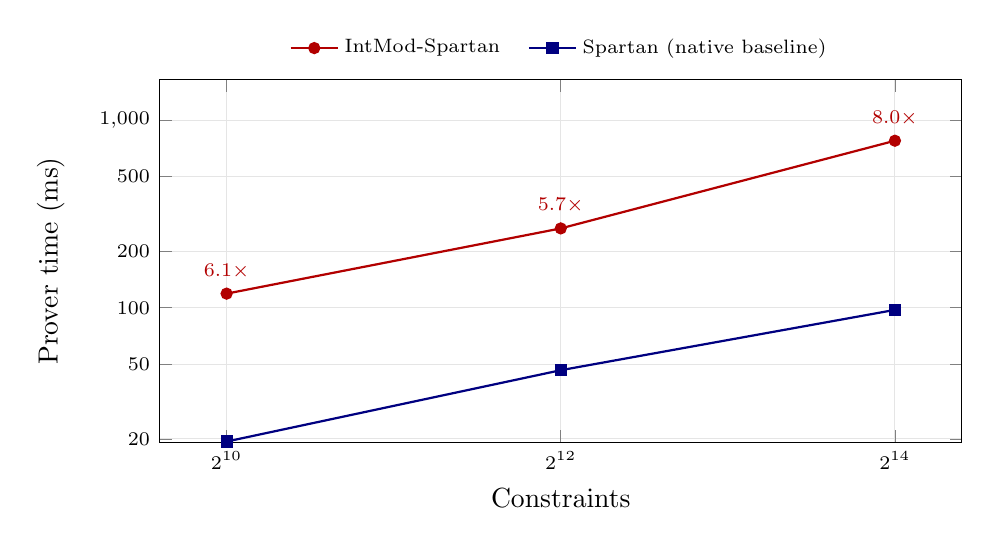
\begin{tikzpicture}
  \begin{axis}[
    scale only axis, width=0.84\linewidth, height=4.6cm,
    yticklabel style={font=\scriptsize, text width=2.4em, align=right},
    xticklabel style={font=\scriptsize},
    ymode=log,
    ytick={20,50,100,200,500,1000}, log ticks with fixed point,
    xtick={10,12,14}, xticklabels={$2^{10}$,$2^{12}$,$2^{14}$},
    xlabel={Constraints}, ylabel={Prover time (ms)},
    grid=both, grid style={gray!20},
    % legend above the axes so it never occludes either series
    legend style={at={(0.5,1.03)}, anchor=south, legend columns=-1,
      font=\scriptsize, draw=none, /tikz/every even column/.append style={column sep=8pt}},
    enlarge y limits={upper, value=0.2},
    error bars/y dir=both, error bars/y explicit,
  ]
    \addplot[ourscolor, thick, mark=*, mark size=1.8pt]
      coordinates {(10,118.955) +- (1.535,1.395) (12,264.896) +- (5.508,6.057) (14,777.339) +- (2.935,4.368)};
    \addlegendentry{IntMod-Spartan}
    \addplot[basecolor, thick, mark=square*, mark size=1.8pt]
      coordinates {(10,19.358) +- (0.083,0.133) (12,46.470) +- (0.406,0.421) (14,97.430) +- (0.289,1.046)};
    \addlegendentry{Spartan (native baseline)}
    \node[above=2pt, ourscolor, font=\scriptsize] at (axis cs:10,118.955) {6.1$\times$};
    \node[above=2pt, ourscolor, font=\scriptsize] at (axis cs:12,264.896) {5.7$\times$};
    \node[above=2pt, ourscolor, font=\scriptsize] at (axis cs:14,777.339) {8.0$\times$};
  \end{axis}
\end{tikzpicture}

\iffull
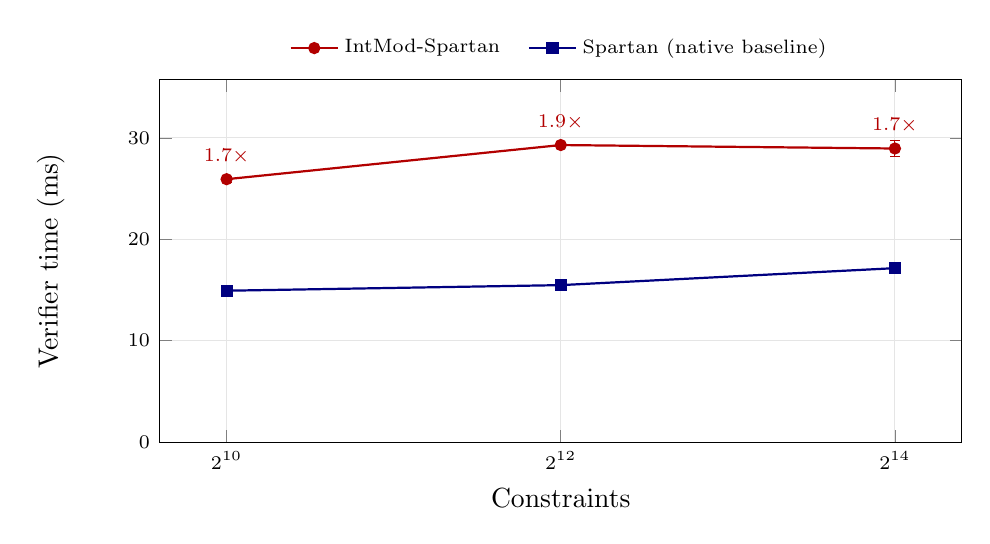
\begin{tikzpicture}
  \begin{axis}[
    scale only axis, width=0.84\linewidth, height=4.6cm,
    yticklabel style={font=\scriptsize, text width=2.4em, align=right},
    xticklabel style={font=\scriptsize},
    ymin=0,
    ytick={0,10,20,30,40},
    xtick={10,12,14}, xticklabels={$2^{10}$,$2^{12}$,$2^{14}$},
    xlabel={Constraints}, ylabel={Verifier time (ms)},
    grid=both, grid style={gray!20},
    % legend above the axes so it never occludes either series
    legend style={at={(0.5,1.03)}, anchor=south, legend columns=-1,
      font=\scriptsize, draw=none, /tikz/every even column/.append style={column sep=8pt}},
    enlarge y limits={upper, value=0.2},
    error bars/y dir=both, error bars/y explicit,
  ]
    \addplot[ourscolor, thick, mark=*, mark size=1.8pt]
      coordinates {(10,25.929) +- (0.198,0.287) (12,29.297) +- (0.434,0.223) (14,28.955) +- (0.307,0.812)};
    \addlegendentry{IntMod-Spartan}
    \addplot[basecolor, thick, mark=square*, mark size=1.8pt]
      coordinates {(10,14.931) +- (0.090,0.075) (12,15.482) +- (0.104,0.112) (14,17.155) +- (0.103,0.069)};
    \addlegendentry{Spartan (native baseline)}
    \node[above=2pt, ourscolor, font=\scriptsize] at (axis cs:10,25.929) {1.7$\times$};
    \node[above=2pt, ourscolor, font=\scriptsize] at (axis cs:12,29.297) {1.9$\times$};
    \node[above=2pt, ourscolor, font=\scriptsize] at (axis cs:14,28.955) {1.7$\times$};
  \end{axis}
\end{tikzpicture}
\fi
